\chapter{THE TEST SUITES}
% !TEX root = hazy2.tex

\section{Introduction}

The code must be completely tested every time anything is changed.
This is done with the test suite that is included in the distribution.
The following pages list the test cases included in the \cdFilename{auto} directory
within the test suite directory \cdFilename{tsuite}.

The test suite contains a series of Perl scripts that automate several tasks.
The \cdFilename{readme\_tests.htm} file included with the tests
describes these scripts.
The script \cdFilename{doc\_tsuite.pl} extracts the test names
and the description of each, and creates two files,
\cdFilename{doc\_tsuite.htm}, a formatted description of each test,
and \cdFilename{doc\_tsuite.txt}, the table that
follows this discussion.

The test cases include a large number of \cdCommand{monitor} commands that allow the code to be
automatically tested every night.
These \cdCommand{monitor} commands have been removed from the examples below.

The simulations form various classes. The names of the classes and their intention
is given in Table \ref{tab:ClassesOfSimulations}.

\begin{table}
\centering
\caption{\label{tab:ClassesOfSimulations}
Keywords used in the Test Suite.}
\begin{tabular}{ c c  }
\hline
Class & Function \\
\hline
Blr & Broad emission line region of AGN \\
Coronal & Collisionally ionized gas with pre-set temperature \\
Dynamics & Flow \\
Function & Test various functions of the code \\
Geometry & Test geometric aspects, aperture command \\
HII & H II regions \\
IGM & Intergalactic medium \\
ISM & Interstellar medium \\
Limit & Test limiting cases \\
NLR & Narrow-lined region of AGN \\
Nova & Aspects of the classical nova explosion \\
Optimizer & Test the optimizers \\
PDR & Photodissociation region \\
PN & Planetary nebulae \\
Stars & Stellar atmospheres \\
\hline
\end{tabular}
\end{table}


\section{Organization of commands}

Commands can (mostly) occur in any order but we have made an effort to
enter them in the order shown below.
This is so that they can be studied to see examples of how to
use the code.

\emph{\# commands controlling continuum}

\emph{\# commands for density \& abundances}

\emph{\# commands controlling geometry}

\emph{\# other commands for details}

\emph{\# commands controlling output}
As indicated, there are the \cdCommand{print} and \cdCommand{save} commands
which control the code's output.

\emph{\# commands giving the monitors}
Each test includes a number of \cdCommand{monitor} commands.
These give values of predicted quantities that the code has
obtained in the past.
Changes to the code may cause predicted values to change,
and if they do the \cdCommand{monitor} command will
announce it.

\section{The Auto Test Suite}

Table \ref{tab:AutoSimulationList} lists the simulations in the 
\cdFilename{auto} test directory.

\begin{table}
\centering
\caption{
The simulations in the auto test suite.}
\begin{tabular}{ c c  }
\hline
Class & Function \\
\hline
\input{../../../tsuite/auto/doc_tsuite.txt}
\hline
\label{tab:AutoSimulationList}
\end{tabular}
\end{table}

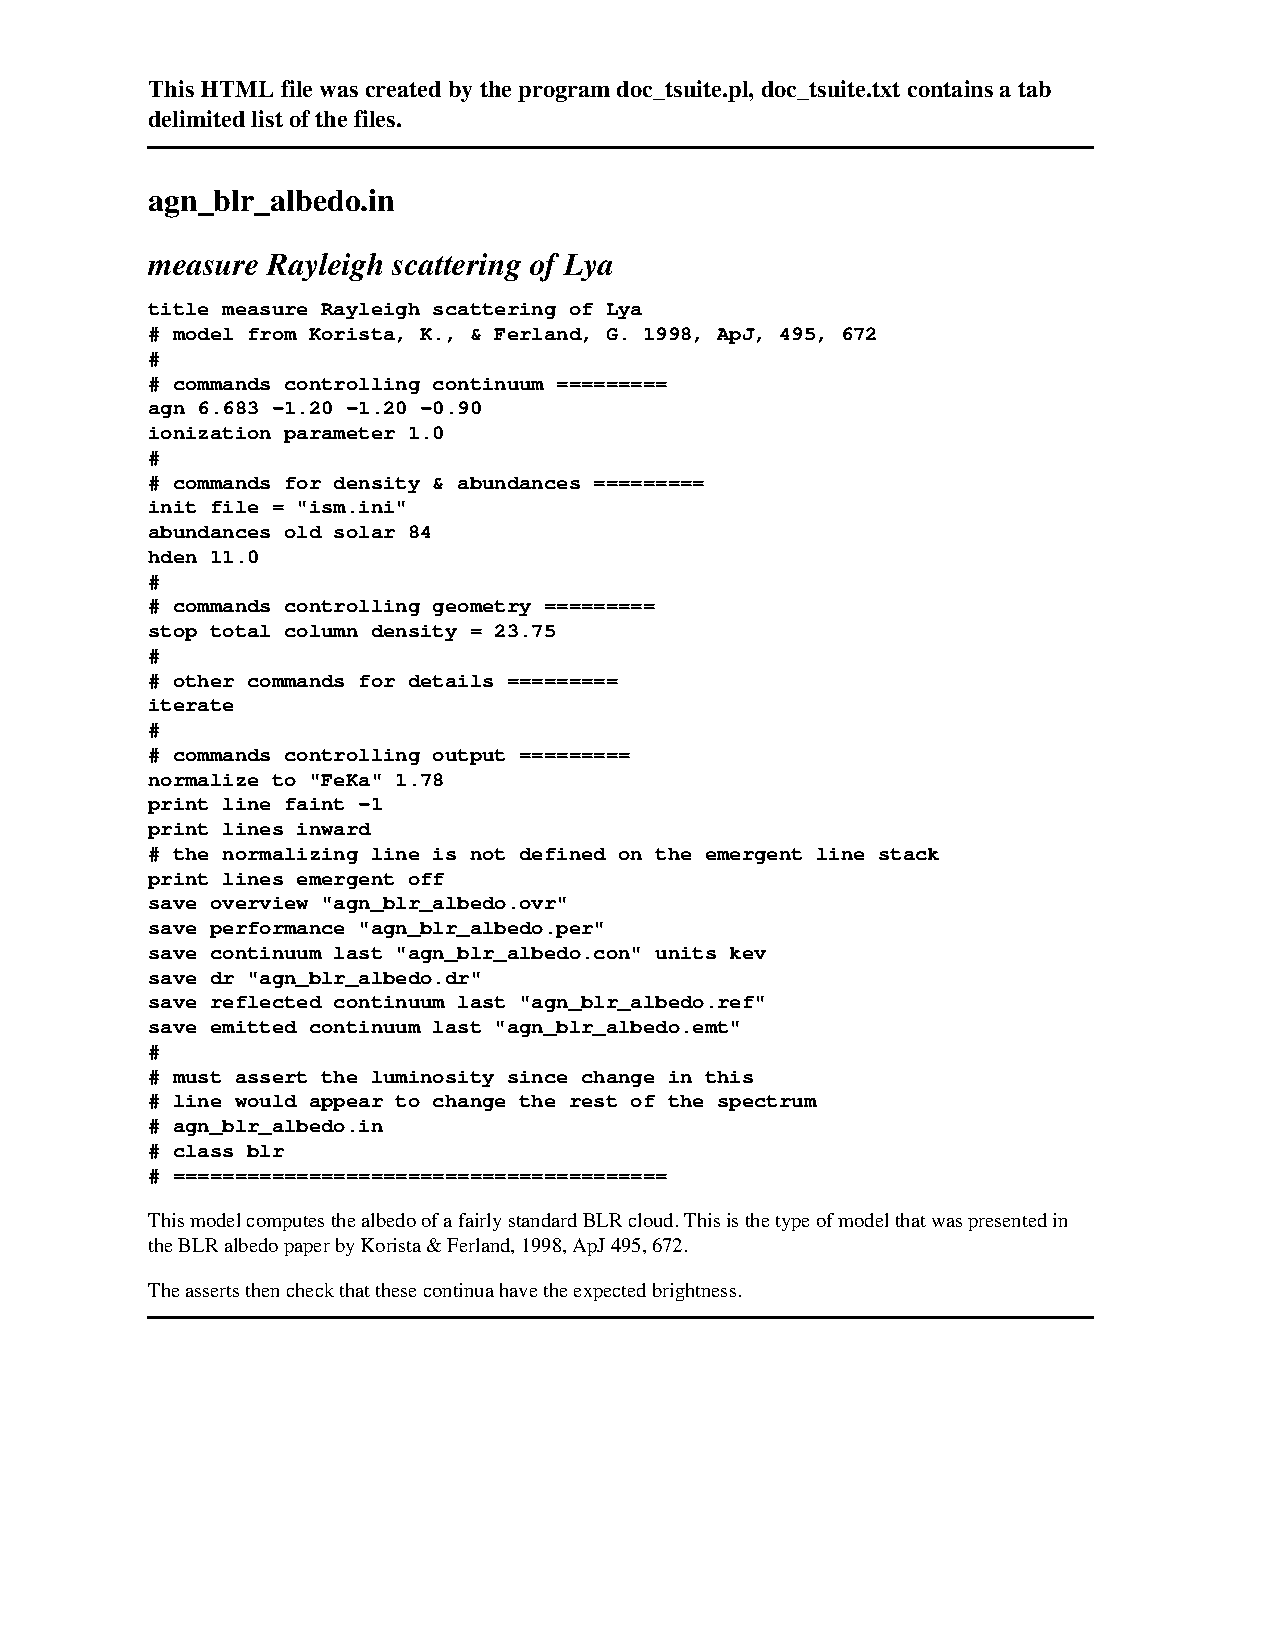
\includepdf[pages=-]{../../../tsuite/auto/doc_tsuite.pdf}

\section{The Slow Test Suite}

Table \ref{tab:SlowSimulationList} lists the simulations in the
\cdFilename{slow} test directory.

\begin{table}
\centering
\caption{
The simulations in the slow test suite.}
\begin{tabular}{ c c  }
\hline
Class & Function \\
\hline
\input{../../../tsuite/slow/doc_tsuite.txt}
\hline
\label{tab:SlowSimulationList}
\end{tabular}
\end{table}

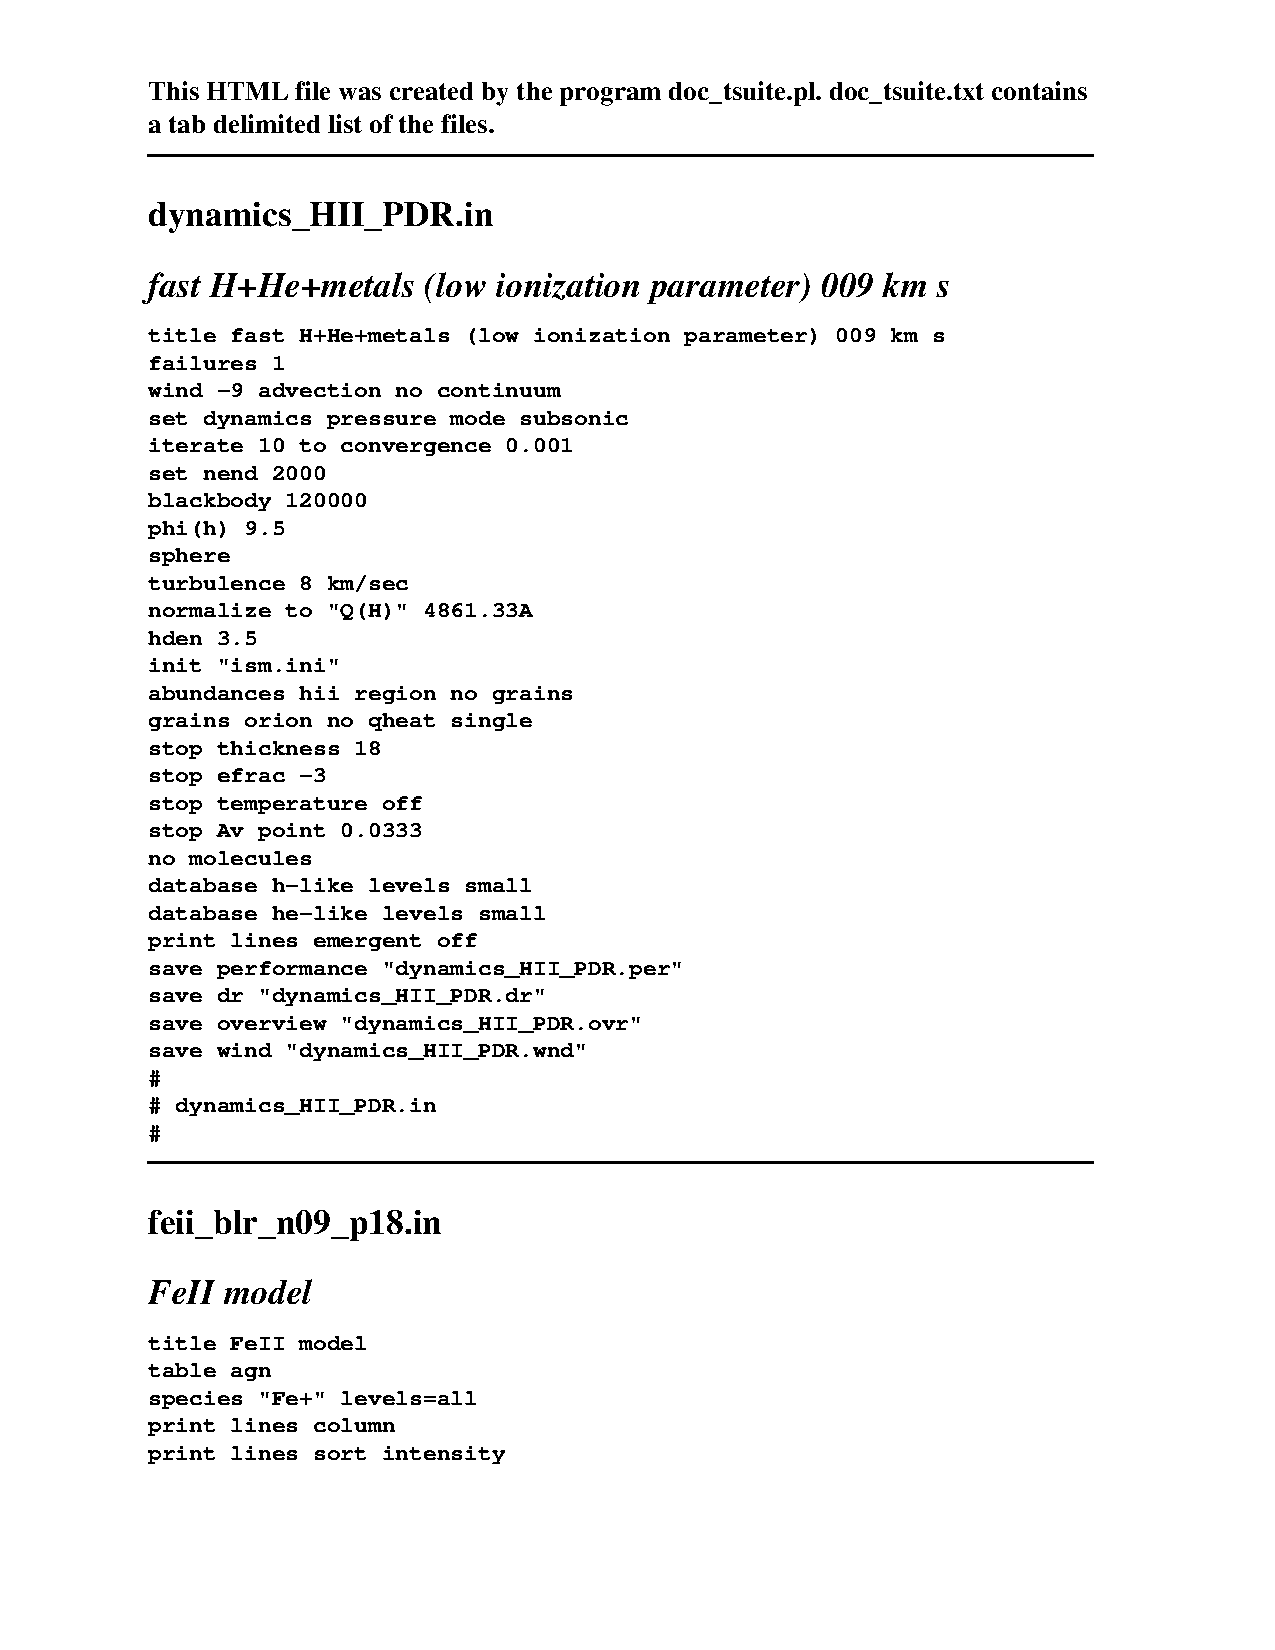
\includepdf[pages=-]{../../../tsuite/slow/doc_tsuite.pdf}


\section{Sample Programs} 
